\documentclass{report}
\usepackage[T1]{fontenc}
\usepackage[utf8]{inputenc}
\usepackage[francais]{babel}
\usepackage{amsmath}
\usepackage{graphicx}
\usepackage[backend=biber,style=authoryear,bibencoding=utf8]{biblatex}
\usepackage[colorlinks,linkcolor=blue]{hyperref}

\addbibresource{biblio.bib}

\begin{document}
\chapter{MRTF-A}
En 2001, \cite{mercher_involvement_2001} 
décrivent une translocation impliquée dans les leucémies aigües mégacaryocytiques. 
Il s'agit de la translocation d'un gène du chromosome 1 sur le chromosome 22, le gène fusion est nommmé One-Twenty-Two-Megakaryocytic-Acute-Leukemia (OTT-MAL). 
Les fonctions des deux gènes qui ont fusionné sont alors inconnues. 

En 2002, deux homologues de la myocardine sont identifiés dans le génome humain par \cite{wang_potentiation_2002} et sont nommés Myocardin-Related Transcription Factor A et B (MRTF-A/B).
MRTF-A correspond au gène du chromosome 22 MAL (ou MKL1) et MRTF-B à un gène du chromosome 16 (MAL16 ou MKL2). 
Un homologue est également découvert chez la souris et nommé Basic, SAP et Coil-coil (BSAC) \parencite{sasazuki_identification_2002}. 

Alors que cette protéine sera appelée dans la suite de cette thèse MRTF-A, elle pourra être identifiée indifféremment comme MAL, MKL1 ou BSAC dans la bibliographie. 

\section{MRTF-A, cofacteur de Serum Response Factor}

La fonction principale des protéines de la famille des myocardines est l'activation du facteur de transcription Serum Response Factor. 

\subsection{Serum Response Factor}

Serum Response Factor est un facteur de transcription qui fait partie de la famille MADS (MCM-1, Agamous, Deficiens, SRF). SRF est présent en un seul exemplaire dans le génome humain mais peut être transcrit en 4 isoformes. 
La protéine SRF comprend un signal de localisation nucléaire (NLS), une boîte MADS composée du site de liaison à l'ADN et d'un domaine de dimérisation, et d'un domaine de transactivation auquel se fixent ses cofacteurs. 

Un dimère SRF se fixe sur une séquence consensus de nucléotides sur l'ADN appelée boîte CArG : CC(A/T)$_{6}$GG, ou sur une séquence CArG-like, qui diffère du consensus d'une seule base, avec une affinité plus faible. Le gène srf contenant lui-même deux boîtes CArG, il est sa propre cible, dans une boucle de rétro-action positive. 

\subsection{Les cofacteurs de SRF : TCF et MRTF}

Serum Response Factor n'est lui-même qu'un transactivateur faible, mais il peut être activé par deux grandes familles de cofacteurs : les Ternary Complex Factors, et les Myocardin-Related Transcription Factors. 

Les deux familles ne sont pas concurrentes pour se lier à SRF : la plupart des sites sur l'ADN sont spécifiques de l'une ou l'autre des familles de cofacteurs (\cite{esnault_rho-actin_2014}). Même lorsque les MRTF sont séquestrées dans le cytoplasme, les TCF ne les remplacent pas sur les sites de liaison à SRF. 

Un ChIP-seq sur des fibroblastes 3T3 a estimé que 921 gènes sont susceptibles d'être régulés par MRTF/SRF en réponse au sérum, et 76 gènes par TCF/SRF (\cite{esnault_rho-actin_2014}), ce qui représente entre 3 et 4\% du génome. Les MRTF sont donc un élément important de la régulation transcriptionnelle, et l'acteur principal de la régulation de SRF. 

\emph{Les autres cofacteurs de SRF ? }

\subsubsection{Ternary Complex Factors}

Elk1, Net et SAP-1 sont trois coactivateurs de SRF de la même famille, les TCF. Ils possèdent un domaine qui leur permet de se lier à des sites spécifiques sur l'ADN (Ets Binding Sites). 
Lorsqu'un site Ets et une boîte CArG sont adjacents, ils forment un Serum Response Element (SRE). La formation d'un complexe TCF-SRF sur un SRE déclenche la transcription du gène cible. 

Les TCF sont phosphorylées et activées par les MAPK (Mitogen Activated Protein Kinases). 


\subsubsection{La famille Myocardine}

\begin{figure}[h!]
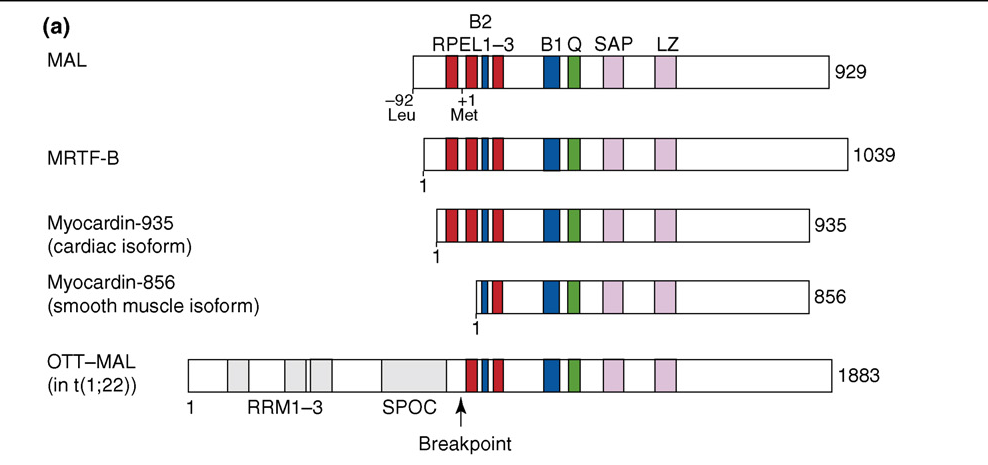
\includegraphics[scale=0.5]{MRTF_famille.png}
\caption{La famille de la myocardine d'après \cite{posern_actin_2006}}
\end{figure}
Cette famille de cofacteurs de SRF comprend la myocardine, MRTF-A et MRTF-B.

La myocardine se présente sous deux isoformes, une forme cardiaque et une forme spécifique au muscle lisse. Les deux sont exclusivement localisées dans le noyau et sont constitutivement actives, en raison de motifs RPEL déficients ou incomplets. 

Les Myocardin-Related Transcription Factors A et B sont exprimées dans un grand nombre de tissus : muscles cardiaques, lisses et squelettiques, neurones, cellules épithéliales, mégacaryocytes \dots Contrairement à la myocardine, les MRTF peuvent être séquestrées dans le cytoplasme, ce qui les empêche d'activer SRF et la transcription. La régulation de la localisation de MRTF est assurée par l'actine, qui peut former un complexe avec la partie N-terminale des MRTF. 

One-Twenty-Two-Megakaryocytic-Acute-Leukemia (OTT-MAL) est la protéine résultant d'une translocation d'un gène du chromosome 1 à côté du gène MRTF-A. La protéine fusion comprend presque toute la protéine MRTF-A excepté la partie N-terminale. 


\section{MRTF-A, indépendamment de SRF}

\subsection{Transition épithélio-mésenchymateuse et domaine SAP}

L'activation de la transcription de la tenascine C en réponse à une stimulation mécanique et à TGF$\beta$ a été liée à MRTF-A (\cite{maier_tenascin-c_2008}). Cependant, cette réponse est indépendante de SRF, ou du domaine liant MRTF-A à SRF (\cite{asparuhova_transcriptional_2011}), elle dépend du domaine SAP. 
S'il est possible que SAP soit capable de lier MRTF-A à l'ADN (\cite{aravind_sapputative_2000}), savoir si MRTF-A est capable d'être un facteur de transcription à lui seul, ou s'il a un partenaire facteur de transcription encore inconnu est une question ouverte. 


\subsection{NF-$\kappa$B}

NF-$\kappa$B est un facteur de transcription impliqué dans les voies de signalisation de l'inflammation. MRTF-A et NF-$\kappa$B peuvent se lier dans le noyau, et s'empêcher l'un l'autre d'activer leurs promoteurs respectifs sur l'ADN (\cite{wang_bone_2012}). 
Cette activité dépend uniquement du domaine C-terminal de MRTF-A, où se trouve le domaine TAD. 
Ainsi l'activation de la voie TNF$\alpha$/NF-$\kappa$B peut être empêchée par l'activation de BMP4/MRTF-A et inversement. 

\section{Structure de MRTF-A}

\begin{figure}[h!]
\center
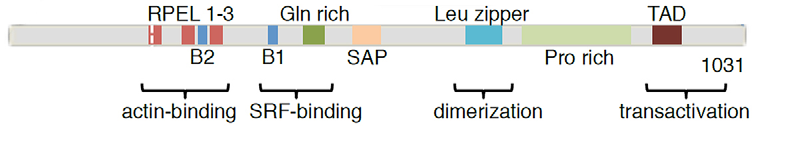
\includegraphics[scale=0.5]{MRTFA_structure.png}
\caption{Structure de MRTF-A \parencite{scharenberg_tgf-_2014}}
\end{figure}
 \subsection{Les motifs RPEL}
 
 La partie N-terminale de MRTF-A contient trois motifs RPEL consécutifs, qui peuvent se lier aux monomères d'actine (\cite{posern_mutant_2004}, \cite{mouilleron_molecular_2008}) avec des affinités variables, les deux premiers motifs se liant plus fortement que le troisième (\cite{guettler_rpel_2008}). La structure détaillée du complexe montre que les trois motifs RPEL se lient à 3 à 5 monomères d'actine selon la concentration en monomères d'actine. (\cite{hirano_sensing_2011}, \cite{treisman_structure_2011}). 
 
 
 \begin{figure}[h!]
 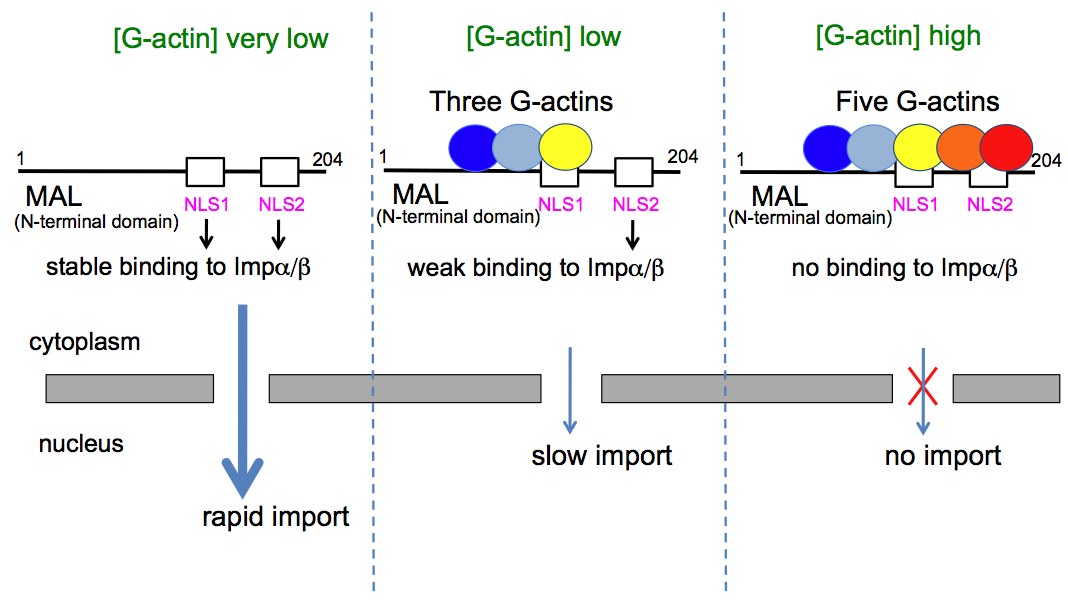
\includegraphics[scale=0.30]{MRTF-A_actines_complexes.png}
 \caption{D'après \cite{hirano_sensing_2011}}
 \end{figure}
 Deux domaines basiques, B2 et B3 sont inclus dans les motifs RPEL et forment un signal de localisation nucléaire (NLS) bipartite (\cite{rajakyla_actin-regulated_2010}). Lorsqu'il n'y a pas d'actine sur les motifs RPEL, ce NLS peut se lier au complexe Importine$\alpha / \beta$ (\cite{hirano_sensing_2011},\cite{rajakyla_actin-regulated_2010}) et MRTF-A est importée dans le noyau de la cellule, où se trouve SRF. En présence de suffisamment de monomères, le NLS est recouvert par l'actine liée aux RPEL, MRTF-A reste cytoplasmique (Posern 2002, \cite{miralles_actin_2003},\cite{posern_mutant_2004}). 
 
 MRTF-A est exportée du noyau par Crm1 (\cite{vartiainen_nuclear_2007},\cite{hayashi_differences_2013}). \emph{Ces deux articles se contredisent sur la question de la liaison à l'actine : le premier prétend qu'elle est indispensable, le second qu'elle empêche l'export} 
 
 Les motifs RPEL sont donc la clé de la régulation de MRTF-A par l'actine : selon la concentration en monomères d'actine, MRTF-A est localisée dans le cytoplasme en cas d'excès et dans le noyau, où se trouve SRF, en cas de manque. Lorsque le domaine RPEL est muté ou absent, la protéine est constitutivement nucléaire (\cite{miralles_actin_2003}), comme la myocardine, dont les motifs RPEL ne sont plus fonctionnels (\cite{guettler_rpel_2008}). 
 
 \subsection{La région basique et SRF}
 \begin{figure}[h!]
 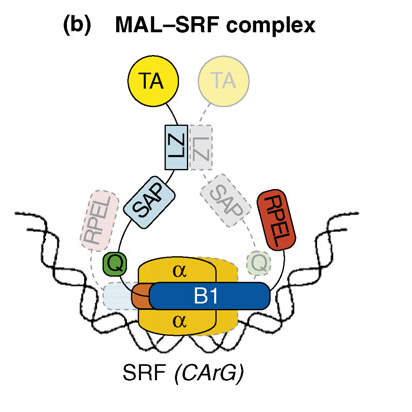
\includegraphics[scale=0.5]{MRTFA_SRF_complex.png}
 \caption{D'après \cite{posern_actin_2006}}
 \end{figure}
 La région B1 est le site de liaison de MRTF-A à SRF. MRTF-A s'attache préférentiellement à SRF en dimère (\cite{miralles_actin_2003}). Le complexe MRTF-A-5actines ne peut pas se lier à SRF et l'activer, la présence de MRTF-A dans le noyau n'est donc pas suffisante pour activer SRF, il faut également que la concentration en G-actine dissocie le complexe (\cite{vartiainen_nuclear_2007}). 
 \subsection{Leucine zipper et oligomérisation}
 MRTF-A/B peuvent former des homo ou des hétérodimères (\cite{miralles_actin_2003}). Un dominant négatif pourra ainsi bloquer une protéine WT dans un hétérodimère non fonctionnel (\cite{selvaraj_megakaryoblastic_2003},\cite{cen_myocardin/mkl_2004}, \cite{li_requirement_2005},\cite{rajakyla_actin-regulated_2010}). La formation des dimères n'est pas indispensable à la fonctionnalité de MRTF-A, les mutations dans cette région réduisent son efficacité sans l'inhiber totalement (\cite{selvaraj_megakaryoblastic_2003}). 
 OTT-MAL est également capable de former des hétérodimères avec les MRTF, et donc de perturber leur équilibre. 
 
 \subsection{SAP}
 
Dans les cellules épithéliales, il a été montré qu'un groupe de gènes est activé par MRTF-A et nécessite particulièrement la zone SAP, tout en étant indépendant de SRF (\cite{asparuhova_transcriptional_2011}, \cite{gurbuz_sap_2014}).
 
 
 \subsection{TAD}
 
 
 
 \subsection{Phosphorylation}
	MRTF-A peut être phosphorylée (\cite{miralles_actin_2003},\cite{cen_myocardin/mkl_2004}).Dans les neurones, la phosphorylation de MRTF-A par ERK1/2 est même la voie principale de régulation de son activité, car la protéine est toujours nucléaire, mais elle n'active SRF qu'une fois phosphorylée (\cite{kalita_role_2006}). Il existe donc au moins une voie d'activation de MRTF indépendante de la régulation de l'actine. 
	
 \subsection{Isoformes}
 \begin{figure}[h!]
 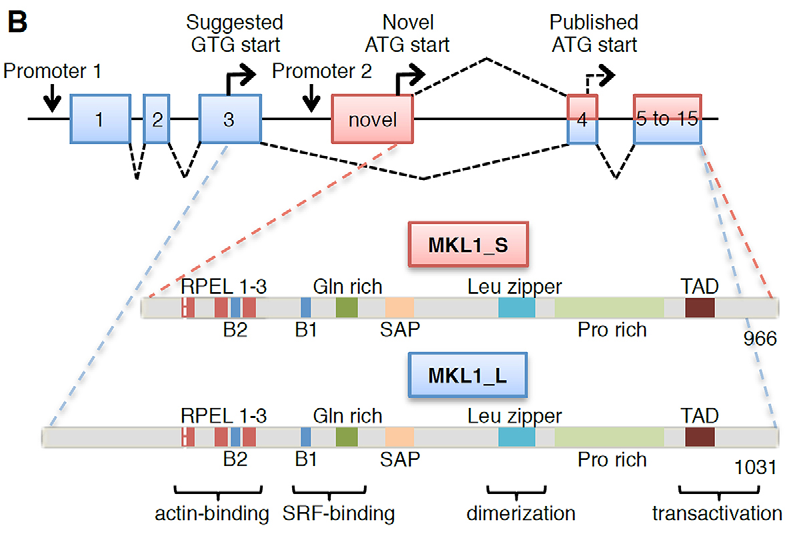
\includegraphics[scale=0.5]{MRTF_isoformes.png}
 \caption{D'après \cite{scharenberg_tgf-_2014} : les deux isoformes de MRTF-A}
 
 \end{figure}
 D'après \cite{scharenberg_tgf-_2014}, il existe 2 isoformes de MRTF-A chez l'humain, une version longue (MRTF-A\_L) et une courte (MRTF-A\_S). La version longue présente 80 acides aminés avant le premier motif RPEL, contre 15 seulement pour la version courte. Cette dernière contient deux TAD de 9 acides aminés (9aaTAD), un à l'extrémité C-terminale, et un à l'extrémité N-terminale spécifique à cet isoforme. Une surexpression de MRTF-A\_S est observée en réponse à TGF-$\beta$ ou à une contrainte cyclique dans les cellules épithéliales. 
 
 



\section{En amont de MRTF-A : voie de signalisation et régulation de l'actine} 


La régulation de l'activité de MRTF-A se fait principalement par sa localisation intracellulaire qui dépend du réservoir d'actine monomérique disponible. 
Lorsque l'actine G est disponible pour former un complexe pentamérique avec MRTF-A, ce complexe est confiné dans le cytoplasme où il ne peut jouer aucun rôle dans la transcription. 
Lorsque l'actine G n'est pas disponible, MRTF-A est importée dans le noyau et peut se lier à SRF pour activer la transcription de ses gènes cibles. 

L'actine est le point de convergence d'une grande diversité de signaux extra-cellulaires ou intracellulaires, biochimiques ou mécaniques, qui vont activer ou inhiber MRTF-A et SRF. 
Ainsi, tout élément qui va perturber la dynamique de l'actine aura des conséquence sur l'activation de MRTF-A : drogues agissant sur l'actine, protéines liées à l'actine (Actin-Binding Proteins, ABP), voies de signalisations, environnement mécanique. 


\subsection{Actines mutantes}

La surexpression d'actine, même sans changer l'équilibre entre les filaments et les monomères, entraîne l'augmentation des monomères disponibles pour former le complexe avec MRTF-A (\cite{miralles_actin_2003},\cite{vartiainen_nuclear_2007}). MRTF-A est alors localisée dans le cytoplasme. 

La surexpression d'une actine-NLS (\cite{vartiainen_nuclear_2007},\cite{posern_mutant_2002}) a le même effet. Lorsque l'export est bloqué par la Leptomycine B, MRTF-A est \emph{de facto} bloquée dans le noyau, mais comme elle reste complexée par l'actine, SRF n'est pas activé. 

Les mutants non-polymérisables comme R62D ont le même effet que la surexpression de l'actine, mais en plus efficace (\cite{posern_mutant_2002},\cite{miralles_actin_2003},\cite{vartiainen_nuclear_2007}, \cite{collard_nuclear_2014}). 

Les mutants qui polymérisent mieux ou qui forment des filaments plus stables déclenchent l'accumulation nucléaire de MRTF-A et l'activation de SRF (\cite{posern_mutant_2004}). 


\subsection{Drogues agissant sur l'actine}

Les drogues agissant sur l'actine sont très souvent utilisées lors des études sur MRTF-A comme contrôles. 

La latrunculine B séquestre les monomères d'actine, empêchant leur incorporation dans les filaments. La liaison Latrunculine-Actine est compatible avec l'incorporation dans le complexe avec MRTF-A (\cite{mouilleron_molecular_2008}). 
L'ajout de latrunculine B permet donc de conserver l'actine hors des filaments et de la rendre disponible pour former un complexe avec MRTF-A, qui est alors séquestré dans le cytoplasme et inactif (\cite{vartiainen_nuclear_2007},\cite{zhao_force_2007},\cite{smith_induction_2013}). 

La cytochalasine D coiffe les microfilaments d'actine à leur extrémité + et empêche leur polymérisation et leur dépolyméristion . 
Contrairement à la latrunculine, elle est incompatible avec la formation du complexe car l'organisation de l'actine dans le complexe actines-RPELs est très différente de l'organisation dans les filaments (\cite{treisman_structure_2011}). 
Par conséquent, la cytochalasine séquestre l'actine hors de portée à la fois des filaments et de MRTF-A, qui est alors importée dans le noyau et activée.(\cite{miralles_actin_2003},\cite{vartiainen_nuclear_2007},\cite{smith_induction_2013}) Le Swinholide A séquestre des dimères d'actine et fonctionne de manière semblable.(\cite{miralles_actin_2003},\cite{vartiainen_nuclear_2007}).

Le Jasplakinolide augmente la polymérisation de l'actine, diminuant la disponibilité de l'actine monomérique et entraînant l'accumulation de MRTF-A dans le noyau (\cite{miralles_actin_2003},\cite{vartiainen_nuclear_2007},\cite{smith_induction_2013}). 


\subsection{Actin-Binding Proteins}

L'équilibre dynamique de polymérisation de l'actine dans la cellule est régulée par de nombreuses protéines impliquées dans d'encore plus nombreuses voies de signalisation. 

De manière générale, les protéines qui vont favoriser la formation ou la stabilité des filaments, comme la profiline, Arp2/3, les formines mDia (\cite{chan_force-induced_2010},\cite{baarlink_nuclear_2013}) ou l'émerine (\cite{ho_lamin_2013}), seront à l'origine d'une accumulation nucléaire de MRTF-A, car elle vont appauvrir les réserves de monomères d'actine. 

Lorsque la voie RhoA est activée, la cofiline est phosphorylée, ce qui l'inactive. L'inactivation de la cofiline stabilise les filaments d'actine, et donc l'accumulation nucléaire de MRTF-A (\cite{zhao_force_2007}). 

La thymosine $\beta$, comme la latrunculine, séquestre les monomères d'actine avec une st\oe chiométrie de 1:1. Mais contrairement à celle-ci, la thymosine $\beta$ empêche l'intégration des monomères dans le complexe avec MRTF-A. Lors d'une surexpression de T$\beta$4, MRTF-A est donc nucléaire et SRF activé (\cite{morita_g-actin_2013}).




\subsection{La voie RhoA}

RhoA (Ras homolog gene family, member A) est une protéine de la famille des petites GTPases dont le rôle est de réguler le cytosquelette d'actine. Ce rôle fait de RhoA une voie de signalisation importante pour MRTF-A. 

RhoA a deux cibles principales : ROCK (Rho-associated coiled-coil-containing protein kinase 1) et les formines mDia (mammalian Diaphanous). La phosphorylation de ROCK entraîne la phosphorylation de LIMK (LIM domain kinase) qui désactive la cofiline. L'activation des formines et le blocage de la cofiline concourent à la formation de filaments d'actine plus longs et plus nombreux et à la réduction des réserves de monomères d'actine. 

La voie RhoA peut être activée par un grand nombre de signaux biochimiques ou mécaniques. ILK (Integrin Linked Kinase) associée à une stimulation mécanique (\cite{maier_tenascin-c_2008}), les androgènes (\cite{schmidt_rhoa_2012}), la thrombopoïétine (\cite{smith_induction_2013}), le sérum (\cite{sotiropoulos_signal-regulated_1999}) et les hormones du rythme circadien (\cite{gerber_blood-borne_2013}) activent la voie de signalisation RhoA/actine/MRTF-A/SRF. 
Une déformation mécanique constante(\cite{albinsson_stretch_2004}, \cite{zhao_force_2007},\cite{chan_force-induced_2010}) ou cyclique (\cite{kuwahara_myocardin-related_2010}), un substrat dur (\cite{huang_matrix_2012}) sont des signeux mécaniques qui vont également activer la voie RhoA. 


\subsection{Un cas particulier : MICAL2}

La signalisation par MRTF-A/B est importante pour le développement des neurones(\cite{kalita_mkls:_2012}), cependant contrairement aux fibroblastes et aux myoblastes, les neurones font l'expérience de contraintes et de réorganisation du cytosquelette beaucoup plus limités. Il n'y a que rarement formation de fibres de stress dans les neurones par exemple. La polymérisation d'actine dans ces cellules n'est pas suffisante pour déclencher la voie MRTF-A de la même manière que dans d'autres types cellulaires. 

Les protéines de la famille MICAL sont capables d'oxyder la methionine 44 de l'actine, ce qui l'empêche de faire partie d'un filament. Cette oxydation peut avoir lieu sur l'actine déjà recrutée dans un filament, causant sa dépolymérisation (\cite{hung_direct_2011}). L'actine oxydée est également sélectivement exportée du noyau, une actine mutante M44Q constitutivement oxydée est confinée dans le cytoplasme (\cite{lundquist_redox_2014}).

MICAL2 est un membre de cette famille particulièrement présent dans le noyau, où il peut contrôler la dépolymérisation de l'actine nucléaire. L'expression d'un mutant dominant négatif de MICAL2 cause l'apparition de longs filaments d'actine dans le noyau, car son activité de dépolymérisation des filaments est interrompue (\cite{lundquist_redox_2014}). 

L'activation de MICAL2 ou sa surexpression entraîne ainsi paradoxalement une accumulation nucléaire de MRTF-A : l'actine du noyau est oxydée, dépolymérisée puis expulsée du noyau, réduisant ainsi la réserve globale d'actine disponible dans le noyau(\cite{lundquist_redox_2014}). 

Lorsque une atrophie musculaire est causée par la dénervation, MICAL2 est sous-exprimée dans les fibres musculaires, ce qui participe au maintient de concentrations importantes d'actine monomérique dans le noyau et donc à l'exclusion de MRTF-A (\cite{collard_nuclear_2014}). 

MICAL2 est donc une voie d'activation de MRTF-A indépendante de RhoA, et donc l'activité se concentre sur le réservoir d'actine nucléaire de la cellule. 


%\section{En aval de MRTF-A : SRF et gènes cibles}
\section{Rôles de MRTF-A}
Depuis sa découverte au début des années 2000, de nombreux rôles de MRTF-A ont été mis en évidence dans des types cellulaires et dans des tissus très divers. 
\subsection{Embryogenèse}

Les MRTF sont exprimées dès le jour 10 du développement de l'embryon (\cite{wang_potentiation_2002}), dans tous les tissus. La délétion de MRTF-B entraîne l'échec de la gastrulation, et donc une fin précoce de l'embryogenèse (\cite{kalita_mkls:_2012}). Au contraire, 60\% des mutants MRTF-A$^{-/-}$ sont viables et atteignent l'âge adulte, les autres étant perdus pendant l'embryogenèse car souffrant de défauts cardiaques. Les mutants survivants sont dépourvus de ces anomalies cardiaques, et vivent jusqu'à l'âge adulte (\cite{li_requirement_2006},\cite{sun_acute_2006}). Cependant, les femelles souffrent d'un défaut de formation de la glande mammaire,  lié à une apoptose précoce des cellules myoépithéliales qui déclenchent l'éjection du lait. Il apparaît donc que chez la souris, tandis que MRTF-B est indispensable à l'embryogenèse, l'absence de MRTF-A peut être compensée dans la plus grande partie des tissus. 
Les souris possédant un gène mutant dominant négatif de MRTF-A sont en revanche de plus petite taille, ne bougent pas et ne survivent que quelques jours, principalement à cause des défauts de musculature de leur diaphragme (\cite{li_requirement_2005}). 

\subsection{Régulation de la masse musculaire}

Serum Response Factor a pour gènes cibles un grand nombre de gènes liés au cytosquelette et à la différenciation musculaire. 

Lorsque SRF est désactivé dans le muscle squelettique de souris adulte ( souris HSA-Cre-ER$^T2$:srf$^{flox/flox}$ ), l'hypertrophie compensatoire de ses muscles est bloquée (\cite{guerci_srf-dependent_2012}). Les cellules satellites sont moins nombreuses, et ne fusionnent pas avec les fibres musculaires. Au contraire, un SRF constitutivement actif protège de l'atrophie liée à une immobilisation ou à une dénervation. 
Suite à une dénervation, MRTF-A est exclue des noyaux des fibres musculaires, et donc incapable d'activer SRF. Une MRTF-A constitutivement nucléaire protège contre l'atrophie induite par la dénervation (\cite{collard_nuclear_2014}). C'est donc la régulation de la localisation de MRTF-A dans les fibres musculaires qui régule l'activité de SRF et l'atrophie ou l'hypertrophie en réponse aux contraintes mécaniques.  


Dans les myoblastes murins C2C12, un dominant négatif MRTF-B, capable d'interférer avec l'activité des deux MRTF, bloque la différenciation musculaire en myotubes et diminue leur taux de duplication (\cite{selvaraj_megakaryoblastic_2003}, \cite{cen_megakaryoblastic_2003}). 
Les souris DN-MRTF-A montrent d'ailleurs un phénotype myopathique. 




\subsection{Transition épithéliale-mésenchymale}

La transition épithélio-mésenchymateuse est le processus par lequel des cellules, sous l'influence de signaux extérieurs, vont perdre leur type épithélial (expression de l'E-cadherine, polarisation, organisation en monocouche jointive \dots) et acquérir un phénotype mésenchymal (expression de N-cadherine, motilité plus importante, fabrication de matrice extra-cellulaire \dots). 
Plusieurs marqueurs de l'EMT, comme la vimentine ou l'actine du muscle lisse $\alpha$Smooth Muscle Actin sont des cibles de SRF. 

La conjonction d'un signal biochimique, TGF $\beta$ (Transforming Growth Factor), et d'un signal mécanique déclenche l'activation de la voie de signalisation RhoA/actine/MRTF-A/SRF. 
Les signaux mécaniques déclencheurs peuvent être très divers, locaux ou globaux, cycliques ou statiques : membranes étirées cycliquement (\cite{maier_tenascin-c_2008}), ilôts de fibronectine  (\cite{gomez_tissue_2010},\cite{connelly_actin_2010}), gels de polyacrylamides de différentes rigidités (\cite{huang_matrix_2012}), microbilles magnétiques recouvertes de collagène (\cite{chan_force-induced_2010}). 

Des anomalies dans la transition épithélio-mésenchymateuse ont été liées aux fibroses pulmonaires et hépatiques.

\subsection{Différenciation des mégacaryocytes}

Les souris MRTF-A KO ont une genèse anormale des mégacaryocytes, les cellules de la moelle osseuse qui sont à l'origine des plaquettes. Les gènes contrôlant la différenciation de ces cellules sont sous le contrôle de SRF. La thrombopoïétine active la voie RhoA/MRTF-A/SRF. 

\subsection{Rythme circadien}

Les plantes, les animaux et même certains organismes unicellulaires possèdent une horloge biologique d'environ 24h, calquée sur l'alternance jour/nuit. Un certain nombre de processus biologiques dépendent des hormones produites par cette horloge dans le cerveau et propagées dans le sang vers l'ensemble des organes, comme le rythme veille/sommeil, la température corporelle, le péristaltisme de l'intestin, la sécrétion des hormones de croissance \dots 

SRF fait partie des facteurs de transcription dont la régulation est sensible au rythme circadien et contient dans ses cibles un certain nombre de gènes régulant le rythme circadien (\cite{esnault_rho-actin_2014}). Une stimulation par ajout de sérum permet de réinitialiser l'horloge biologique.

Dans le foie de rats et de souris, la polymérisation de l'actine est maximale au lever du jour (fin de période d'activité pour les rongeurs nocturnes) et minimale au crépuscule (\cite{gerber_blood-borne_2013}). De manière synchronisée, les MRTF sont nucléaires et SRF est activé au lever du jour, et les MRTF sont cytoplasmiques et SRF désactivé au coucher du soleil. Le niveau d'expression de l'actine et de MRTF ne varie pas au cours de la journée. Chez l'humain, espèce diurne, ce rythme est inversé mais également présent. 



\subsection{MRTF-A et cancers}
Le rôle de MRTF-A dans l'invasion, les métastases et la prolifération cancéreuse est complexe. 
Dans l'exemple du cancer du sein, on a attribué à MRTF-A un rôle antiprolifératif en tant que facteur de transcription de l'Eplin$\alpha$ (Epithelial protein lost in Neoplasm), protéine qui est inversement corrélée avec la mortalité et l'invasion cancéreuse ( \cite{leitner_epithelial_2010}).
Cependant, dans les cancers du sein sensibles aux \oe strogènes, l'activation de MRTF-A favorise la transition vers un type insensible au contrôle hormonal (\cite{kerdivel_activation_2014}) et MRTF et SRF sont nécessaires à l'adhésion, à la motilité et à l'invasion dans des lignées issues de cancers du sein et de mélanomes (\cite{medjkane_myocardin-related_2009}).  
Les gènes contrôlés par MRTF-A indépendamment de SRF semblent être liés à un mauvais pronostic (\cite{gurbuz_sap_2014}). 

\cite{leitner_mal/mrtf-controls_2011} montre bien le rôle complexe que peut avoir la régulation d'un élément du cytosquelette dans différents contextes : MRTF-A augmente l'adhésion dans deux types cellulaires, des cellules épithéliales non-invasives et des cellules tumorales de cancer du sein, mais l'effet sur la motilité est opposé dans les deux types. Dans les cellules mammaires épithéliales, l'augmentation de l'adhésion causée par la surexpression de MRTF-A cloue les cellules sur place : l'adhésion est trop forte et les cellules ne sont plus capables de se détacher pour avancer. Inversement, l'adhésion était le facteur limitant dans les cellules tumorales. Avec la surexpression de MRTF-A, elles adhèrent mieux et se déplacent plus efficacement. 

L'activation de la voie RhoA/MRTF/SRF est liée à l'agressivité des tumeurs de la prostate (\cite{schmidt_rhoa_2012}), et une mutation du premier intron de MRTF-A a été identifiée dans des triplets homozygotes dont deux ont développé un lymphome de Hodgkin (\cite{bjorkholm_development_2013}), sans qu'un lien précis soit établi. 

\subsubsection{Le cas particulier d'OTT-MAL}

OTT-MAL est une protéine issue de la fusion d'un gène du chromosome 1 également nommé RBM15, qui régule le facteur de transcription RBPJ (recombination signal binding protein for immunoglobulin $\kappa$ J region), et MRTF-A sur le chromosome 22, qui régule SRF. La présence de cette mutation a été reliée à des leucémies à mégacaryoblastes (\cite{mercher_involvement_2001}). 
La protéine fusion est toujours localisée dans le noyau et active SRF (\cite{descot_ott-mal_2008}), elle peut former des hétérodimères avec MRTF-A et donc interférer avec les protéines saines. Mais c'est l'activation de RBPJ qui est déterminante pour ses propriétés oncogènes dans les mégacaryocytes (\cite{mercher_ott-mal_2009}). 

\subsection{Réorganisation de la chromatine}

En plus de son rôle de régulateur de la transcription des cibles de SRF, plusieurs effets de MRTF-A sur l'organisation de la chromatine ont été mis en évidence. L'activation de MRTF-A et de différents mutants montre une augmentation de l'acétylation de l'histone H3, de la quantité d'euchromatine et de l'activité transcriptionnelle (\cite{flouriot_actin/mkl1_2014}). Cette fonction de MRTF-A nécessite son domaine C-terminal. 
Les fibroblastes 3T3 cultivés sur des motifs de grande taille montrent une plus grande quantité de MRTF-A dans le noyau, associée à une histone déacétylase HDAC3 séquestrée dans le cytoplasme et une plus grande activité transcriptionnelle (\cite{jain_cell_2013}). 

L'histone méthyltransférase SMYD3 coopère avec MRTF-A, sans interaction direct, pour réguler la transcription du gène MYL9 codant pour la Myosin Light Chain (\cite{luo_histone_2014}). 


\newpage

\printbibliography
\end{document}